\documentclass[12pt,a4paper]{report}

% =========================================================================
% DINH DANG CHUNG - THEO MAU CAC BAO CAO ASSIGNMENT TRUOC
% =========================================================================
\usepackage{fontspec}
\setmainfont{Times New Roman}
\usepackage[top=2.5cm,bottom=2.5cm,left=3cm,right=2cm]{geometry}
\usepackage{amsmath,amssymb}
\usepackage{graphicx}
\usepackage{booktabs,tabularx,array}
\usepackage{float}
\usepackage{xcolor}
\usepackage{tikz}
\usetikzlibrary{calc,shapes.geometric}
\usepackage{hyperref}
\usepackage{fancyhdr}
\usepackage{titlesec}
\usepackage{caption}
\usepackage{enumitem}
\usepackage{listings}

\renewcommand{\chaptername}{Chương}
\renewcommand{\contentsname}{Mục Lục}
\renewcommand{\listfigurename}{Danh Mục Hình}
\renewcommand{\listtablename}{Danh Mục Bảng}
\renewcommand{\figurename}{Hình}
\renewcommand{\tablename}{Bảng}
\renewcommand{\bibname}{Tài Liệu Tham Khảo}

\graphicspath{{images/generated/}{images/deploy/}}
\hypersetup{
    colorlinks=true,
    linkcolor=blue!80!black,
    citecolor=green!60!black,
    urlcolor=blue!70!black,
    pdftitle={Bao Cao Assignment 07 - Knowledge Graph, RAG va Agent},
    pdfauthor={khoipv.447}
}

\definecolor{reportblue}{RGB}{0,45,145}
\definecolor{backcolour}{rgb}{0.96,0.97,0.98}
\lstdefinestyle{mystyle}{
    backgroundcolor=\color{backcolour},
    basicstyle=\ttfamily\footnotesize,
    breaklines=true,
    keepspaces=true,
    showstringspaces=false,
    numbers=left,
    numberstyle=\tiny\color{black!55},
    numbersep=5pt,
    frame=single,
    rulecolor=\color{black!20},
    captionpos=b
}
\lstset{style=mystyle}

\titleformat{\chapter}[display]
  {\normalfont\bfseries\color{reportblue}}
  {\filleft\Large\bfseries\chaptertitlename\ \thechapter}
  {1ex}
  {\titlerule\vspace{1ex}\filright\LARGE}
  [\vspace{1ex}\titlerule]
\titleformat{\section}
  {\normalfont\Large\bfseries\color{blue!70!black}}
  {\thesection}{1em}{}
\titleformat{\subsection}
  {\normalfont\large\bfseries\color{black!85}}
  {\thesubsection}{1em}{}

\pagestyle{fancy}
\fancyhf{}
\fancyhead[R]{\small\itshape Assignment 07: Knowledge Graph, RAG và Agent}
\fancyfoot[C]{\thepage}
\renewcommand{\headrulewidth}{0.4pt}
\renewcommand{\footrulewidth}{0.4pt}
\setlength{\headheight}{14pt}

\newcommand{\codeinline}[1]{\texttt{\detokenize{#1}}}

\begin{document}

% =========================================================================
% TRANG BIA
% =========================================================================
\hypersetup{pageanchor=false}
\begin{titlepage}
\thispagestyle{empty}
\begin{tikzpicture}[remember picture,overlay]
    \draw[line width=1.1pt]
      ($(current page.north west)+(1.45cm,-1.35cm)$)
      rectangle
      ($(current page.south east)+(-1.45cm,1.35cm)$);
    \draw[line width=0.35pt]
      ($(current page.north west)+(1.60cm,-1.50cm)$)
      rectangle
      ($(current page.south east)+(-1.60cm,1.50cm)$);
\end{tikzpicture}
\begin{center}
    \textbf{\fontsize{16}{20}\selectfont
    HỌC VIỆN CÔNG NGHỆ BƯU CHÍNH VIỄN THÔNG}\\[0.15cm]
    \textbf{\fontsize{15}{19}\selectfont KHOA CÔNG NGHỆ THÔNG TIN 1}\\[0.25cm]
    \rule{4cm}{0.4pt}

    \vspace{0.75cm}
    
\begin{tikzpicture}
        \node[text=red!80!black,font=\bfseries\fontsize{30}{34}\selectfont,inner sep=1pt] (ptit) {PTIT};
        \node[star,star points=5,star point ratio=2.2,fill=yellow!85!orange,
              draw=yellow!60!black,minimum size=0.72cm,inner sep=0pt]
              at ($(ptit.north)+(0.18cm,-0.06cm)$) {};
        \draw[red!80!black,line width=1.1pt]
            ($(ptit.south west)+(-0.10cm,-0.18cm)$) --
            ($(ptit.south east)+(0.10cm,-0.18cm)$);
        \draw[red!80!black,line width=0.45pt]
            ($(ptit.south west)+(-0.10cm,-0.25cm)$) --
            ($(ptit.south east)+(0.10cm,-0.25cm)$);
    \end{tikzpicture}

    \vspace{0.55cm}
    \textbf{\fontsize{17}{21}\selectfont BÁO CÁO MÔN HỌC}\\[0.25cm]
    \textbf{\fontsize{17}{21}\selectfont PHÁT TRIỂN CÁC HỆ THỐNG THÔNG MINH}\\[0.40cm]
    \textbf{\fontsize{17}{21}\selectfont ASSIGNMENT 07}\\[0.22cm]
    \textbf{\fontsize{15}{19}\selectfont KNOWLEDGE GRAPH, RAG VÀ AGENT}

    \vspace{0.9cm}
    \begin{tabular}{>{\bfseries}p{3.8cm}p{6.2cm}}
        Họ tên: & Phan Văn Khôi \\
        Mã sinh viên: & B23DCCN447 \\
        Lớp: & D23CTPM01-B \\
        Giảng viên: & PGS. TS. Trần Đình Quế \\
    \end{tabular}

    \vfill
    \textbf{\fontsize{14}{18}\selectfont Hà Nội -- 2026}
\end{center}
\end{titlepage}
\hypersetup{pageanchor=true}

\pagenumbering{roman}
\tableofcontents
\clearpage
\listoffigures
\clearpage
\listoftables
\clearpage
\pagenumbering{arabic}

\chapter*{Thông Tin Project}
\addcontentsline{toc}{chapter}{Thông Tin Project}
\noindent\textbf{GitHub project:} \url{https://github.com/KhoiF/PTHTTM}

\medskip
\noindent Báo cáo này tổng hợp hai notebook và hai ứng dụng cục bộ của Assignment 07:
\begin{itemize}[leftmargin=*]
    \item \textbf{Amazon Stock Price:} \codeinline{amazon_kb_rag_agent.ipynb} và \codeinline{deploy.py};
    \item \textbf{diabetes\_large:} \codeinline{diabetes_kb_rag_agent.ipynb} và \codeinline{deploy.py}.
\end{itemize}
Hai notebook thực hiện khảo sát dữ liệu, xây Knowledge Graph (KG), lập chỉ mục Retrieval-Augmented
Generation (RAG), rồi kiểm tra agent. Hai file deploy cung cấp giao diện dòng lệnh và web Flask trên
localhost. Các số liệu, hình EDA và câu trả lời minh họa dưới đây được lấy từ output đã lưu của notebook.

% =========================================================================
% CHUONG 1
% =========================================================================
\chapter{Cơ Sở Lý Thuyết Về Knowledge Graph Và RAG}

\section{Lịch sử và vai trò}
Các hệ cơ sở tri thức biểu diễn sự kiện bằng thực thể và quan hệ đã được nghiên cứu trước thời đại
large language model. Semantic Web phát triển các chuẩn để mô tả và liên kết tài nguyên bằng dữ liệu có
cấu trúc. Năm 2012, Google giới thiệu Knowledge Graph trong tìm kiếm nhằm xử lý thực thể cùng quan hệ
của chúng thay vì chỉ khớp chuỗi ký tự \cite{google_kg}. Năm 2020, Lewis và cộng sự giới thiệu
Retrieval-Augmented Generation, kết hợp truy xuất nguồn tri thức với mô hình sinh văn bản
\cite{lewis_rag}.

Trong bài tập này, KG đóng vai trò một knowledge base (KB) có thể truy vấn theo khóa và quan hệ. RAG
biến dữ liệu thành các đoạn văn có nguồn, tìm đoạn liên quan đến câu hỏi và cung cấp chúng cho mô hình
ngôn ngữ. Agent chọn công cụ phù hợp với câu hỏi và trả kèm nguồn, giúp người đọc kiểm tra được dữ kiện.

\section{Knowledge Graph và bộ ba tri thức}
Một KG có thể mô tả bằng $G=(V,E)$, trong đó $V$ là tập nút và
$E\subseteq V\times R\times V$ là tập cạnh có nhãn quan hệ thuộc $R$.
Bộ ba $(s,p,o)$ gồm chủ thể, quan hệ và đối tượng. Ví dụ:
\begin{equation}
    (\texttt{year:2023},\;\texttt{has\_month},\;\texttt{month:2023-12}).
\end{equation}
Mỗi node còn có thuộc tính số hoặc văn bản. Chẳng hạn, node phiên AMZN ngày 05/12/2023 lưu
\codeinline{Close = 146.880005}, còn node nhóm giới tính nữ của diabetes lưu số bản ghi, số nhãn 1
và tỷ lệ. Graph được cài bằng \codeinline{networkx.DiGraph}. Khóa node ổn định và tên quan hệ tường
minh giúp tránh nhập nhằng khi truy vấn.

Quy trình tạo KB gồm kiểm tra schema CSV, chuẩn hóa khóa, xây node/cạnh, nạp thuộc tính và đối chiếu
với phép tính trực tiếp trên CSV. KB chỉ phản ánh những sự kiện được đưa vào graph. Truy vấn một ngày
không có phiên hoặc một nhóm không có trong CSV phải báo thiếu dữ liệu.

\section{Retrieval-Augmented Generation}
RAG gồm hai giai đoạn chính. Khi chuẩn bị dữ liệu, hệ thống chuyển CSV thành tài liệu ngắn có ID nguồn
và lập chỉ mục. Khi nhận câu hỏi, hệ thống truy xuất tài liệu liên quan, đặt chúng vào prompt và yêu
cầu mô hình sinh câu trả lời dựa trên ngữ cảnh đó:
\begin{equation}
    \text{CSV}\rightarrow\text{Documents}\rightarrow\text{Index}
    \xrightarrow{\text{Question}}\text{Top-}k\text{ evidence}
    \rightarrow\text{LLM}\rightarrow\text{Answer + Sources}.
\end{equation}
Hai ứng dụng dùng Qwen3-0.6B cục bộ cho bước sinh \cite{qwen3_card}. Model chỉ được nạp khi câu hỏi
thật sự đi vào nhánh RAG và được giữ trong bộ nhớ cho các câu hỏi tiếp theo.

\section{TF-IDF và độ tương đồng cosine}
Notebook dùng \codeinline{TfidfVectorizer} với \codeinline{analyzer="char_wb"}, n-gram ký tự độ dài
3--5 để xử lý câu hỏi tiếng Việt xen tên cột tiếng Anh. TF-IDF tăng trọng số cho những cụm đặc trưng
của tài liệu và giảm trọng số của cụm xuất hiện phổ biến. Với vector câu hỏi $q$ và tài liệu $d$,
điểm xếp hạng là:
\begin{equation}
    \operatorname{cosine}(q,d)=\frac{q\cdot d}{\lVert q\rVert_2\lVert d\rVert_2}.
\end{equation}
Hệ thống lấy nhiều nhất bốn tài liệu có điểm từ $0{,}10$. Ngưỡng này chỉ là điều kiện liên quan về
mặt văn bản; nó không bảo đảm nội dung được truy xuất đủ để trả lời mọi câu hỏi. Nếu không có tài liệu
đạt ngưỡng, agent thông báo thiếu bằng chứng.

\section{Agent điều phối có kiểm soát}
Agent áp dụng quy tắc từ trên xuống: phát hiện khóa ngày hoặc nhóm để tra graph, dùng CSV cho phép
tính tổng hợp, và dùng RAG cho câu hỏi mô tả. Các giá trị thống kê được tạo bằng phép tính trên dữ liệu
hoặc thuộc tính graph; LLM diễn đạt tài liệu truy xuất. Đầu ra gồm ba trường
\codeinline{answer}, \codeinline{sources} và \codeinline{tools}. Trường \codeinline{tools} cho biết
nhánh thực sự đã chạy, ví dụ \codeinline{knowledge_graph} hoặc cặp
\codeinline{rag_retrieval}, \codeinline{local_llm}.

% =========================================================================
% CHUONG 2
% =========================================================================
\chapter{Thiết Kế Hệ Thống Và Dữ Liệu}

\section{Hai dataset và phạm vi hỏi đáp}
\begin{table}[H]
\centering
\caption{Tổng quan hai CSV gốc}
\label{tab:datasets}
\begin{tabularx}{\textwidth}{lrrX}
\toprule
\textbf{Dataset} & \textbf{Bản ghi} & \textbf{Cột CSV} & \textbf{Thông tin chính} \\
\midrule
Amazon Stock Price & 6.684 & 7 & Date, OHLC, Adj Close, Volume; lịch sử 15/05/1997--05/12/2023 \\
diabetes\_large & 100.000 & 9 & Đặc điểm nhân khẩu, chỉ số và nhãn \codeinline{diabetes} nhị phân \\
\bottomrule
\end{tabularx}
\end{table}

File Amazon được đọc theo ngày và sắp tăng dần. File diabetes có chín cột gốc; hàm nạp tạo thêm
\codeinline{age_group} theo bốn khoảng 0--17, 18--39, 40--59 và 60 tuổi trở lên. Vì vậy DataFrame
sau xử lý có mười cột. Các khoảng tuổi chỉ dùng để mô tả dữ liệu, không phải ngưỡng y khoa.

\section{Schema graph và nguồn văn bản}
\begin{table}[H]
\centering
\caption{Biểu diễn KG và corpus RAG của hai bài toán}
\label{tab:representation}
\begin{tabularx}{\textwidth}{p{3cm}XX}
\toprule
 & \textbf{Amazon Stock Price} & \textbf{diabetes\_large} \\
\midrule
Node & AMZN, năm, tháng, phiên giao dịch & Dataset, nhóm thống kê, kết quả nhãn 0/1 \\
Quan hệ & \codeinline{has_year}, \codeinline{has_month}, \codeinline{has_session} & \codeinline{has_cohort}, \codeinline{positive_count}, \codeinline{negative_count} \\
Thuộc tính & OHLC, Adj Close, Volume của phiên & Số bản ghi, số nhãn 1, tỷ lệ của nhóm \\
Tài liệu RAG & Tổng quan, một tài liệu mỗi phiên, một tài liệu mỗi tháng & Tổng quan và một tài liệu mỗi nhóm \\
\bottomrule
\end{tabularx}
\end{table}

Không tạo node theo từng người bệnh trong diabetes. Điều này giữ KG ở mức thống kê, phù hợp với
câu hỏi tổng hợp và tránh suy diễn rằng hai bản ghi có đặc điểm giống nhau là cùng một cá nhân.
Mỗi tài liệu có ID cố định như \codeinline{AMZN:2023-12-05},
\codeinline{AMZN:month:2023-12} hoặc \codeinline{DIABETES:gender:Female}.

\section{Chỉ mục, sinh câu trả lời và định tuyến}
\begin{table}[H]
\centering
\caption{Cấu hình thực tế trong hai file deploy}
\label{tab:config}
\begin{tabularx}{\textwidth}{p{4.2cm}X}
\toprule
\textbf{Thành phần} & \textbf{Cấu hình} \\
\midrule
Graph & \codeinline{networkx.DiGraph}, tạo khi khởi tạo agent \\
Chỉ mục & TF-IDF ký tự, n-gram 3--5; ma trận sparse trong bộ nhớ \\
Truy xuất & Cosine similarity; tối đa 4 tài liệu, điểm tối thiểu $0{,}10$ \\
Mô hình sinh & \codeinline{Qwen/Qwen3-0.6B}; tối đa 180 token mới; không bật thinking mode \\
Deploy & Flask bind \codeinline{127.0.0.1}; CLI và \codeinline{POST /api/chat} \\
\bottomrule
\end{tabularx}
\end{table}

Amazon ưu tiên câu hỏi có hai ngày, một ngày, tháng, năm hoặc ``mới nhất'' để tra graph/CSV.
diabetes ưu tiên từ chối yêu cầu chẩn đoán, liệt kê schema và trả thống kê theo nhóm hoặc toàn bộ
dataset. Câu hỏi mô tả mới đi vào RAG. Prompt yêu cầu Qwen3 trả lời bằng tiếng Việt và chỉ dùng
ngữ cảnh truy xuất; giao diện luôn hiển thị ID nguồn bên cạnh câu trả lời.

% =========================================================================
% CHUONG 3
% =========================================================================
\chapter{Thực Nghiệm Trên Amazon Stock Price}

\section{Khảo sát và phân bố dữ liệu}
Notebook đọc 6.684 phiên từ 15/05/1997 đến 05/12/2023, không có ngày giao dịch trùng hoặc giá trị
thiếu ở các cột bắt buộc. Bốn ô trong Hình~\ref{fig:amazon_eda} lần lượt thể hiện diễn biến Close,
histogram Close, phân bố phần trăm thay đổi mỗi phiên và Volume theo thời gian. Phân bố biến động được
cắt hiển thị tại $\pm20\%$ để phần trung tâm dễ quan sát; dữ liệu gốc không bị cắt khi xây KB.
\begin{figure}[H]
    \centering
    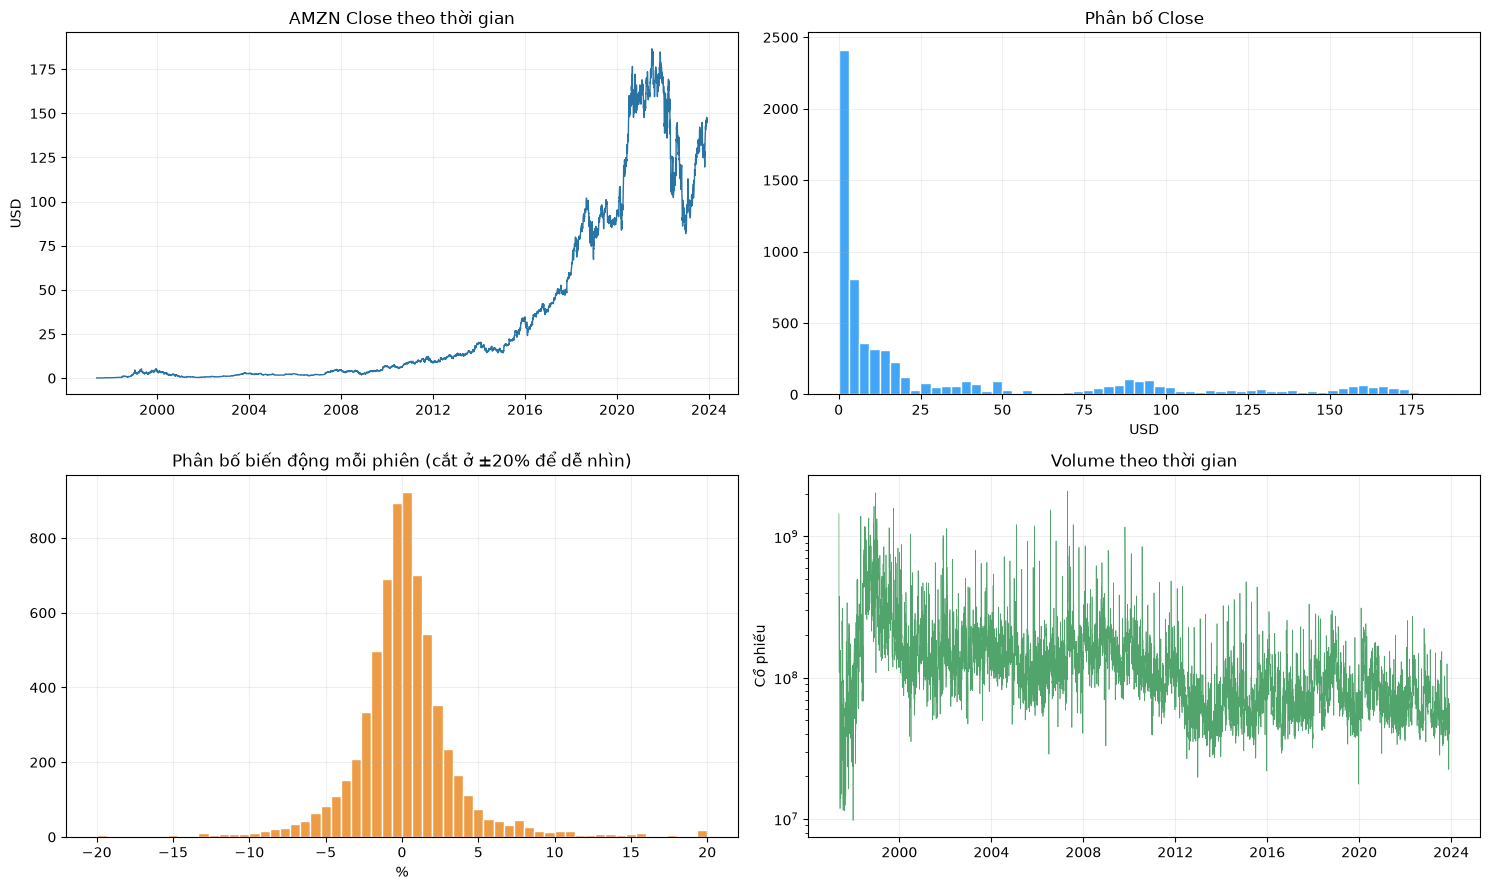
\includegraphics[width=\textwidth]{amazon_eda_overview.png}
    \caption{EDA Amazon Stock Price xuất từ output notebook Assignment 07}
    \label{fig:amazon_eda}
\end{figure}
Giá theo thời gian có xu hướng và phạm vi thay đổi lớn. Vì thế, histogram gộp toàn bộ giai đoạn
chỉ mô tả tập quan sát lịch sử, không phải phân phối giá cố định cho các năm tiếp theo.

\section{Kết quả xây graph và chỉ mục RAG}
KG Amazon có \textbf{7.032 node} và \textbf{7.031 cạnh}. Một đường đi mẫu nối AMZN đến nút
năm 1997, nút tháng 05/1997, rồi đến phiên ngày 15/05/1997.
Truy vấn node ngày 05/12/2023 cho \codeinline{Close = 146.880005}; đối chiếu với CSV trong notebook
cho cùng giá trị, báo cáo làm tròn thành 146,88 USD.

Corpus có \textbf{7.005 tài liệu}; ma trận TF-IDF có kích thước
$7.005\times58.345$. Với truy vấn về Amazon tháng 12/2023, tài liệu
\codeinline{AMZN:month:2023-12} được xếp đầu trong ví dụ notebook với điểm cosine $0{,}2643$.
Các tài liệu lân cận có thể được trả thêm vì truy vấn mang nhiều cụm chung như ``Amazon'', ``Close''
và ``Volume''; vì vậy cần đọc ID nguồn cùng nội dung.

\section{Câu hỏi kiểm chứng}
\begin{table}[H]
\centering
\caption{Đầu ra agent Amazon đã lưu trong notebook}
\label{tab:amazon_questions}
\begin{tabularx}{\textwidth}{p{5.0cm}Xl}
\toprule
\textbf{Câu hỏi} & \textbf{Kết quả} & \textbf{Công cụ} \\
\midrule
Close ngày 05/12/2023? & 146,8800 USD; nguồn \codeinline{AMZN:2023-12-05} & KG \\
Close từ 01 đến 05/12/2023? & 3 phiên; trung bình 146,2500 USD; min 144,8400; max 147,0300 USD & CSV \\
Phiên cuối trong dữ liệu? & 05/12/2023; Close 146,8800 USD & KG \\
Tóm tắt dữ liệu Amazon AMZN? & 6.684 phiên từ 15/05/1997 đến 05/12/2023; nguồn \codeinline{AMZN:overview} & RAG + LLM \\
\bottomrule
\end{tabularx}
\end{table}
Giá ở phiên cuối chỉ là giá cuối \emph{trong CSV}; ứng dụng không truy cập giá thị trường hiện tại và
không dự báo giá tương lai trong Assignment 07.

% =========================================================================
% CHUONG 4
% =========================================================================
\chapter{Thực Nghiệm Trên diabetes\_large}

\section{Khảo sát, nhãn và phân bố}
CSV có \textbf{100.000 bản ghi} và chín cột gốc. Notebook ghi nhận \textbf{3.854 dòng trùng toàn
bộ thuộc tính}; các dòng này vẫn được giữ để thống kê phản ánh đúng tập dữ liệu cung cấp. Không có
giá trị thiếu ở chín cột được dùng. Nhãn \codeinline{diabetes=1} có 8.500 bản ghi, tương đương
\textbf{8,50\%}; nhãn 0 có 91.500 bản ghi.

Hình~\ref{fig:diabetes_eda} cho thấy phân bố nhãn, tuổi, BMI, HbA1c, glucose và tỷ lệ nhãn 1 theo
giới tính. Sự khác nhau giữa các nhóm là mô tả của dataset, không xác lập quan hệ nhân quả.
\begin{figure}[H]
    \centering
    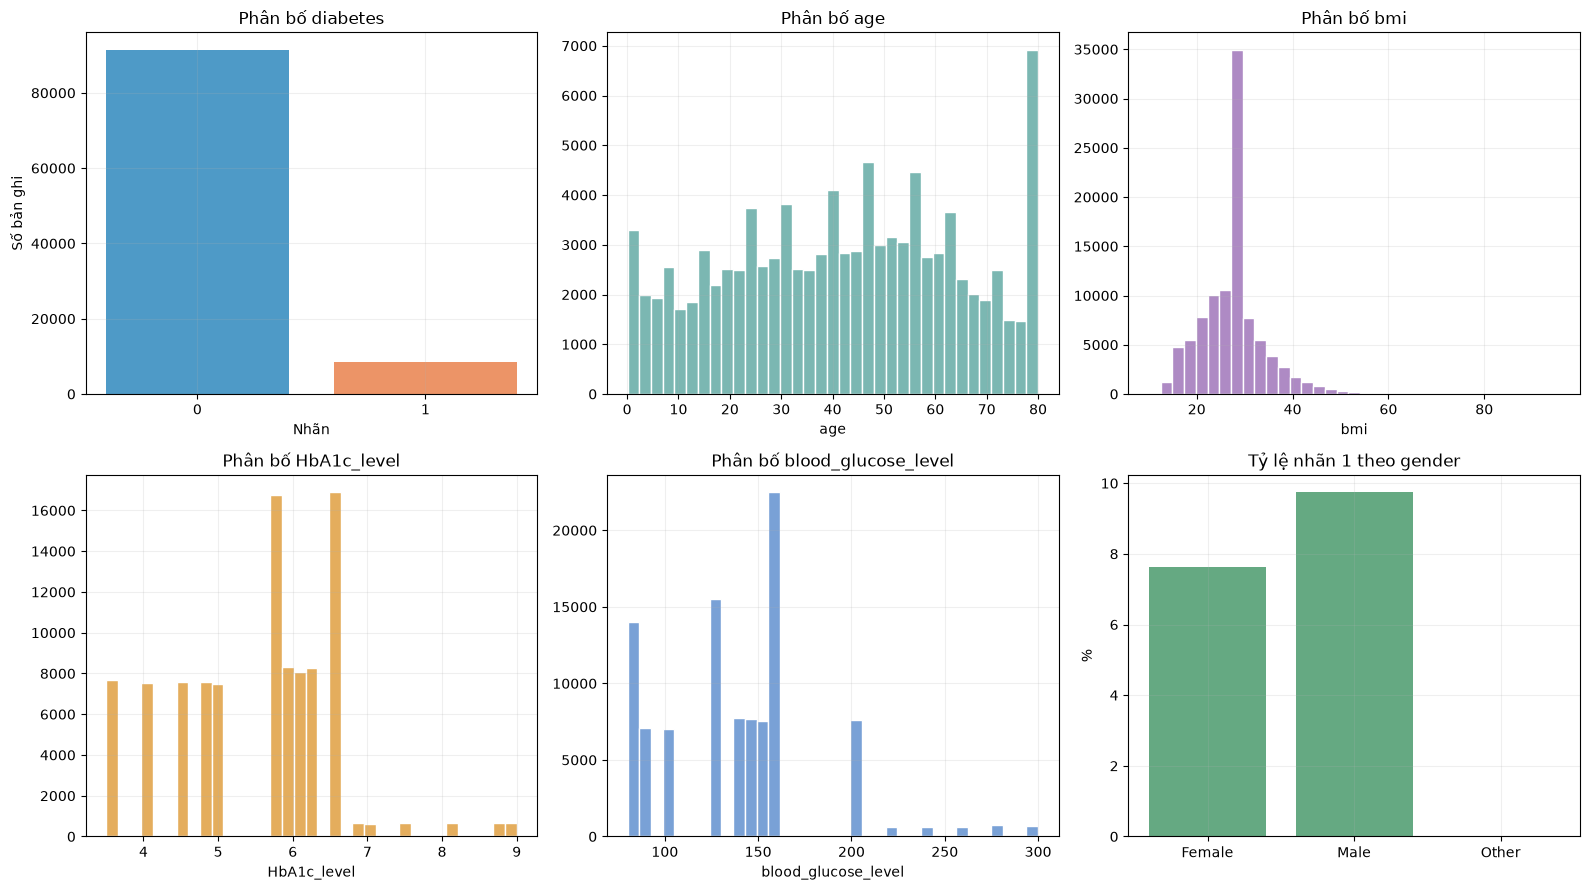
\includegraphics[width=\textwidth]{diabetes_eda_overview.png}
    \caption{EDA diabetes\_large xuất từ output notebook Assignment 07}
    \label{fig:diabetes_eda}
\end{figure}

\section{Kết quả xây graph và chỉ mục RAG}
KG gồm \textbf{20 node} và \textbf{51 cạnh}. Ví dụ node
\codeinline{cohort:gender:Female} nối từ node dataset, rồi nối đến hai node kết quả nhãn.
Thuộc tính node cho biết 58.552 bản ghi nữ, 4.461 bản ghi nhãn 1 và tỷ lệ 7,62\%.
Notebook đối chiếu số lượng và số nhãn 1 với phép lọc trực tiếp từ CSV.

Corpus có \textbf{18 tài liệu}; ma trận TF-IDF có kích thước $18\times1.351$.
Trong ví dụ truy xuất \emph{``Tóm tắt diabetes gender Female''}, tài liệu
\codeinline{DIABETES:gender:Female} đứng đầu với điểm $0{,}4447$. Tài liệu nhóm Male và Other
cũng xuất hiện trong top-k do có nhiều thuật ngữ chung; điểm truy xuất không được xem là tỷ lệ bệnh.

\section{Câu hỏi kiểm chứng}
\begin{table}[H]
\centering
\caption{Đầu ra agent diabetes\_large đã lưu trong notebook}
\label{tab:diabetes_questions}
\begin{tabularx}{\textwidth}{p{4.6cm}Xl}
\toprule
\textbf{Câu hỏi} & \textbf{Kết quả} & \textbf{Công cụ} \\
\midrule
Tỷ lệ diabetes ở nữ? & 58.552 bản ghi, 4.461 nhãn 1, tỷ lệ 7,62\% & KG \\
Tỷ lệ toàn dataset? & 100.000 bản ghi, 8.500 nhãn 1, tỷ lệ 8,50\% & CSV \\
Tỷ lệ nhóm 60+? & 25.055 bản ghi, 4.932 nhãn 1, tỷ lệ 19,68\% & KG \\
Tóm tắt diabetes\_large? & 100.000 bản ghi; 8.500 nhãn 1 và 91.500 nhãn 0; nguồn \codeinline{DIABETES:overall} & RAG + LLM \\
\bottomrule
\end{tabularx}
\end{table}
Ứng dụng chỉ trình bày thống kê của tập quan sát. Đầu ra không dùng để chẩn đoán, ước lượng nguy cơ
cá nhân hoặc quyết định điều trị.

% =========================================================================
% CHUONG 5
% =========================================================================
\chapter{Triển Khai Agent Trên Localhost}

\section{CLI, web và API}
Mỗi \codeinline{deploy.py} khởi tạo graph và chỉ mục khi agent được tạo. Chế độ CLI dùng
\codeinline{--question}; chế độ web dùng \codeinline{--web}. Flask nhận
\codeinline{POST /api/chat} với JSON chứa trường \codeinline{question} và trả về
\codeinline{answer}, \codeinline{sources}, \codeinline{tools}. Input rỗng hoặc sai kiểu được từ chối.
Ứng dụng bind \codeinline{127.0.0.1}; cổng mặc định là 8007 cho Amazon và 8008 cho diabetes.

\begin{lstlisting}[language=bash,caption={Khoi dong hai giao dien web tu thu muc goc project}]
python "src/Assignment 07/Amazon Stock Price/deploy.py" --web --port 8007
python "src/Assignment 07/diabetes_large/deploy.py" --web --port 8008
\end{lstlisting}
Mỗi lệnh cần chạy ở một terminal riêng. Mở \url{http://127.0.0.1:8007} hoặc
\url{http://127.0.0.1:8008}, nhập câu hỏi rồi xem câu trả lời cùng nguồn và công cụ.
Qwen3 được tải từ cache khi gặp câu hỏi đi vào nhánh RAG; lần tải model đầu tiên cần kết nối mạng.
Các câu hỏi tra graph hoặc thống kê CSV không cần gọi LLM.

\section{Giao diện Amazon: câu hỏi graph và RAG}
Với câu hỏi về \codeinline{Close} ngày 05/12/2023, agent dùng graph và hiển thị nguồn
\codeinline{AMZN:2023-12-05}. Câu hỏi tóm tắt dùng RAG, sau đó gọi LLM cục bộ.
Đầu ra ghi hai công cụ \codeinline{rag_retrieval} và \codeinline{local_llm}.
Nguồn là \codeinline{AMZN:overview}.

\begin{figure}[H]
    \centering
    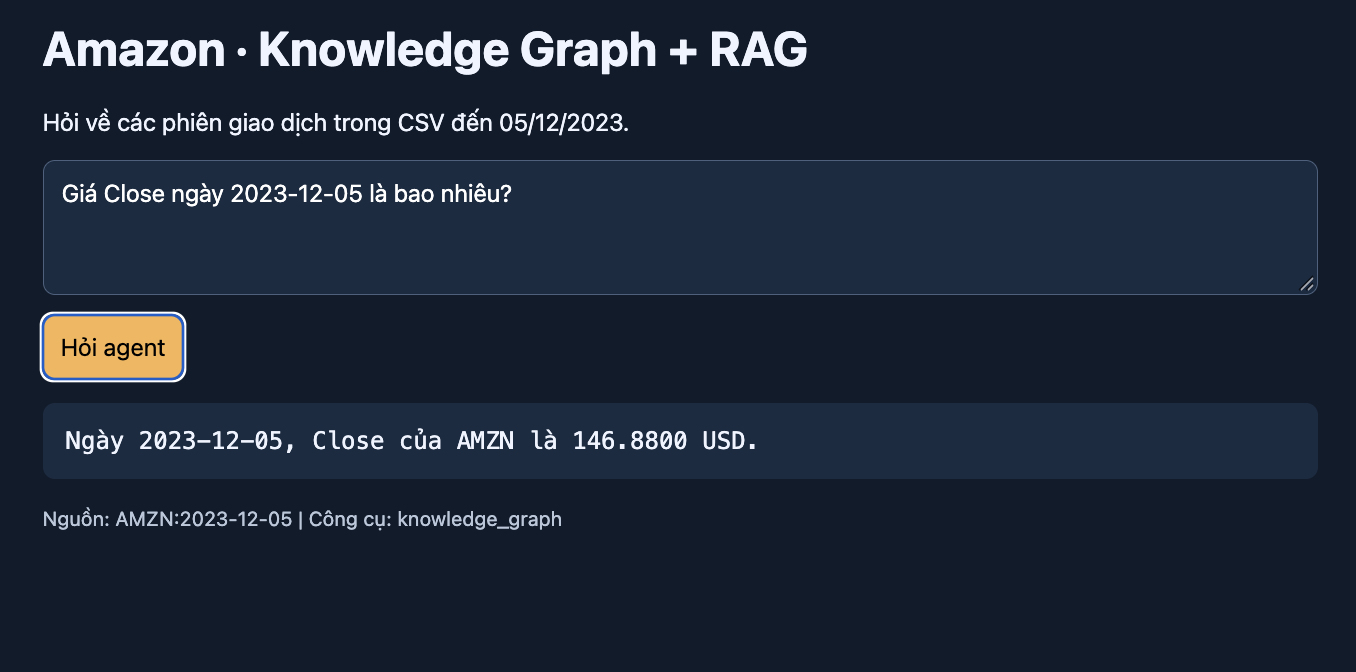
\includegraphics[width=0.94\textwidth]{images/deploy/amazon_kb.png}
    \caption{Giao diện Amazon trả lời câu hỏi Close ngày 05/12/2023 bằng Knowledge Graph}
    \label{fig:amazon_deploy_kb}
\end{figure}

\begin{figure}[H]
    \centering
    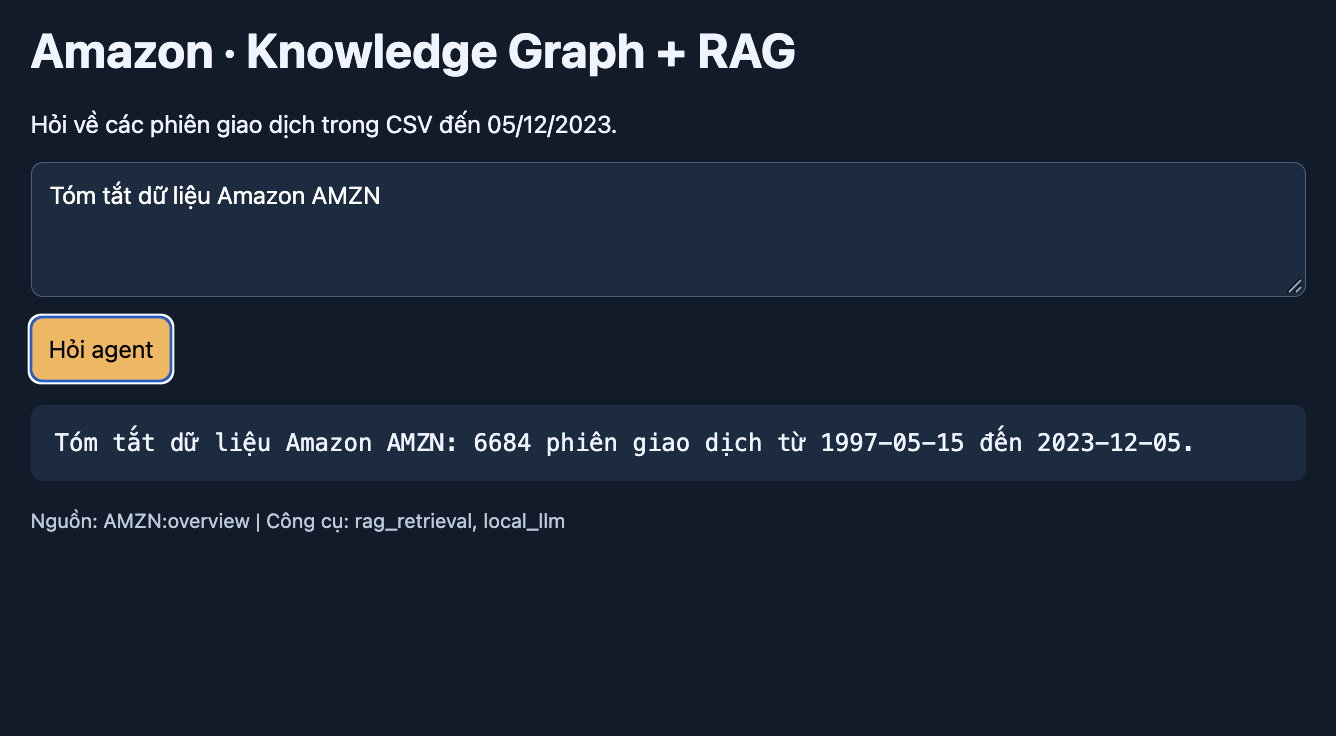
\includegraphics[width=0.94\textwidth]{images/deploy/amazon_rag.png}
    \caption{Giao diện Amazon trả lời câu hỏi tóm tắt bằng RAG và Qwen3}
    \label{fig:amazon_deploy_rag}
\end{figure}

\section{Giao diện diabetes\_large: câu hỏi graph và RAG}
Với câu hỏi tỷ lệ nhãn 1 ở nữ, agent đọc node nhóm. ID nguồn được hiển thị là:
\begin{center}
\codeinline{DIABETES:gender:Female}
\end{center}

Với câu hỏi tóm tắt dataset, agent truy xuất tài liệu tổng quan
\codeinline{DIABETES:overall} và dùng Qwen3 để diễn đạt câu trả lời.

\begin{figure}[H]
    \centering
    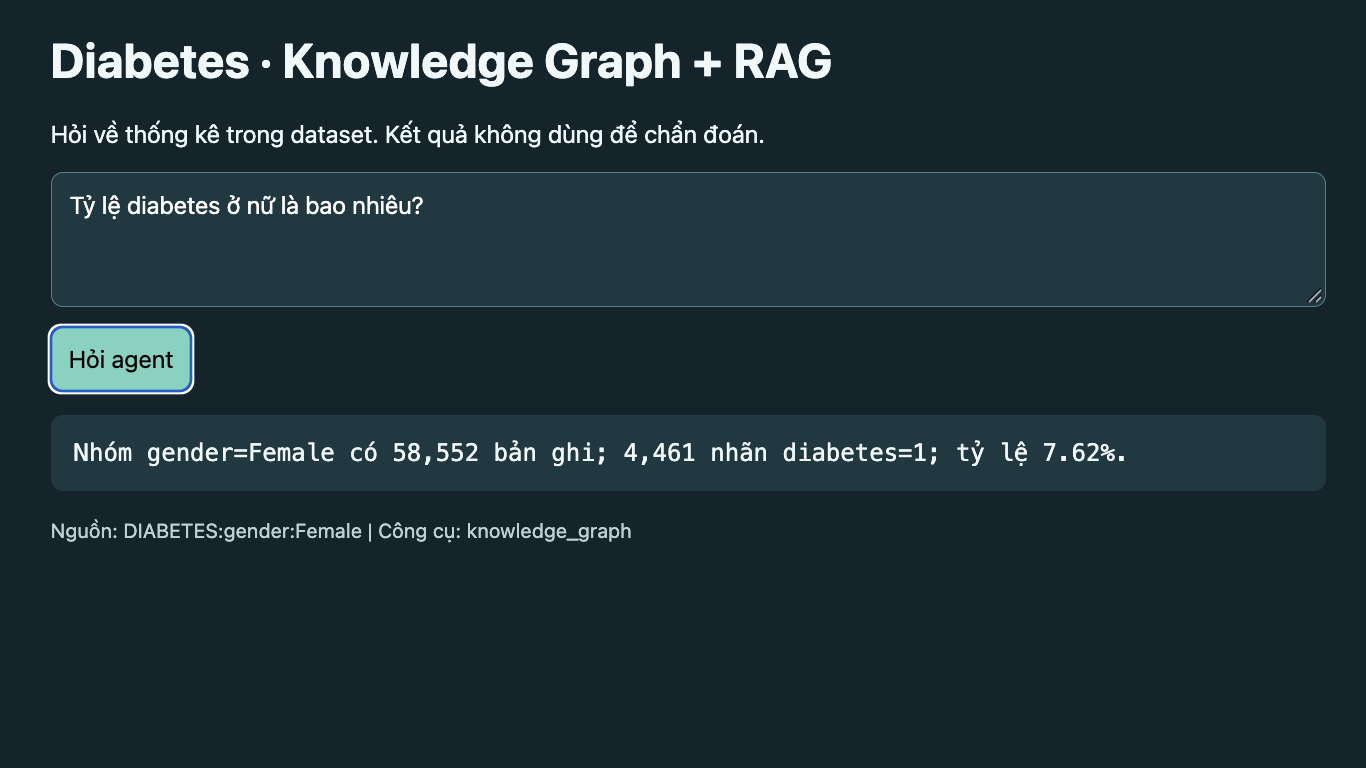
\includegraphics[width=0.94\textwidth]{images/deploy/diabetes_kb.png}
    \caption{Giao diện diabetes trả lời tỷ lệ nhãn 1 ở nữ bằng Knowledge Graph}
    \label{fig:diabetes_deploy_kb}
\end{figure}

\begin{figure}[H]
    \centering
    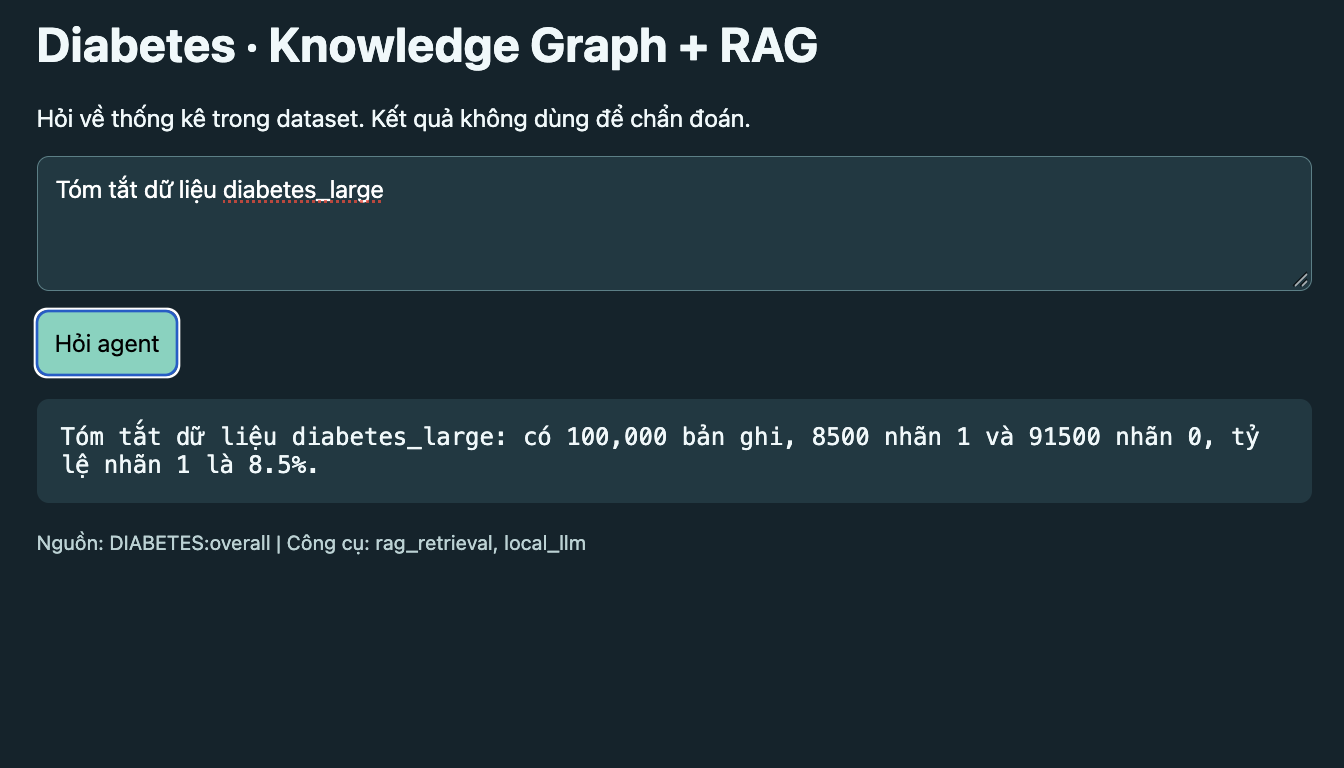
\includegraphics[width=0.94\textwidth]{images/deploy/diabetes_rag.png}
    \caption{Giao diện diabetes trả lời câu hỏi tóm tắt bằng RAG và Qwen3}
    \label{fig:diabetes_deploy_rag}
\end{figure}

% =========================================================================
% CHUONG 6
% =========================================================================
\chapter{Đánh Giá, Giới Hạn Và Kết Luận}

\section{Kiểm chứng khả năng tái lập}
Hai notebook đều có 21 cell và đã chạy hết các cell code, gồm cell
\codeinline{RUN_LOCAL_LLM=True}; output được lưu trong notebook, không có cell lỗi.
Các câu hỏi kiểm chứng số liệu được đối chiếu với CSV. Kiểm tra API bao gồm trang web, payload hợp
lệ, payload sai kiểu, ngày không có phiên, câu hỏi ngoài phạm vi và yêu cầu chẩn đoán. Trong các ví dụ
RAG, đầu ra có \codeinline{tools} chứa \codeinline{rag_retrieval} và \codeinline{local_llm}, cùng
ID tài liệu nguồn.

\section{Giới hạn và hướng phát triển}
\begin{itemize}[leftmargin=*]
    \item TF-IDF ký tự dựa vào mức giống văn bản; truy vấn diễn đạt xa từ vựng corpus có thể không
          tìm được tài liệu phù hợp. Bài tập chưa có bộ câu hỏi gán nhãn để đo Recall@$k$ hoặc
          groundedness một cách hệ thống.
    \item Qwen3-0.6B có thể rút gọn hoặc diễn đạt thiếu chi tiết. ID nguồn giúp kiểm tra lại, nhưng
          không tự chứng minh rằng mọi mệnh đề trong câu trả lời đều đúng.
    \item Giá Amazon dừng ở 05/12/2023. Dữ liệu diabetes là dữ liệu quan sát với nhãn mất cân bằng;
          tỷ lệ nhóm không phải quan hệ nhân quả hoặc công cụ chẩn đoán.
    \item Flask development server phục vụ demo localhost. Khi triển khai cho nhiều người dùng,
          cần bổ sung giới hạn request, quản lý tài nguyên model và cơ chế vận hành phù hợp.
\end{itemize}

\section{Kết luận}
Assignment 07 xây hai hệ hỏi đáp cục bộ trên dữ liệu bảng bằng cách kết hợp Knowledge Graph,
thống kê CSV và RAG. Graph xử lý câu hỏi có khóa rõ ràng, phép tính trên CSV giữ độ chính xác cho
câu hỏi số, còn RAG cung cấp ngữ cảnh có nguồn cho câu hỏi mô tả. Hai notebook và hai ứng dụng CLI/web
cho thấy luồng từ khảo sát dữ liệu, biểu diễn tri thức, truy xuất đến trả lời bằng agent. Việc giữ
nguồn và nêu giới hạn của từng dataset là điều kiện cần để sử dụng kết quả đúng mục đích.

\begin{thebibliography}{9}
\bibitem{google_kg}
Google Research, ``New Challenges in Computer Science Research,'' 2012.
\url{https://research.google/blog/new-challenges-in-computer-science-research/}.

\bibitem{lewis_rag}
P. Lewis et al., ``Retrieval-Augmented Generation for Knowledge-Intensive NLP Tasks,'' 2020.
\url{https://arxiv.org/abs/2005.11401}.

\bibitem{qwen3_card}
Qwen, ``Qwen3-0.6B Model Card.''
\url{https://huggingface.co/Qwen/Qwen3-0.6B}.
\end{thebibliography}

\end{document}
